\begin{definition}{Relative Extrema}
    \begin{itemize}
      \item Relative Extremal-Stelle $x_0$ $\quad \Longrightarrow \quad$ Minimal-/Maximalstelle
    
      \item Relatives Extremum $y_0$ $\quad \Longrightarrow \quad$ Maximum/Minimum
    
      \item Relativer Extremal-Punkt $P_0 = (x_0, y_0)$ $\quad \Longrightarrow \quad$ Hoch-/Tiefpunkt
    
    \end{itemize}
\end{definition}

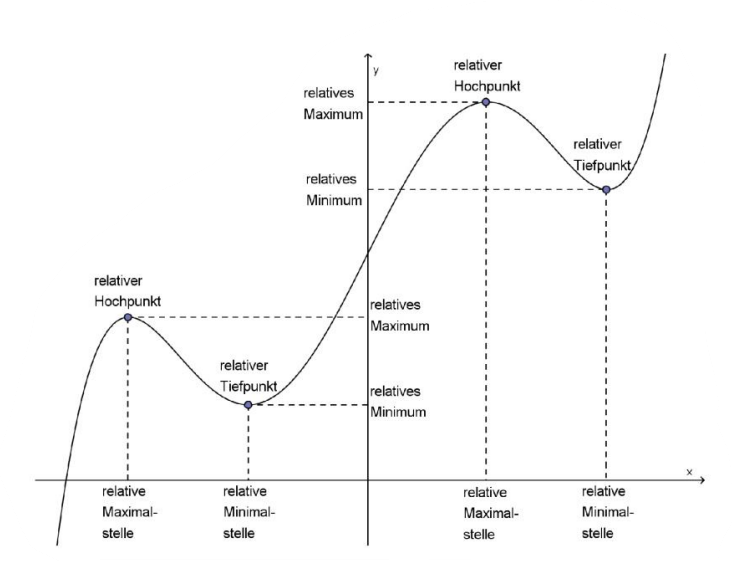
\includegraphics[scale=0.45]{Analysis1/zsf/Images/Differential/relative maxima.png}

\begin{KR}{Vorgehen relative Extrema} von $f(x) = y$:
    \begin{enumerate}
	\item Bestimme $f'(x)$ (Erste Ableitung)
	\item Bestimme NST von $f'(x)$\\
		$f'(x) = 0$ $ \Rightarrow$ $x$ lokales Extremum
	\item Bestimme $f''(x)$ (Zweite Ableitung)
		\begin{itemize}
			\item $f''(x) = 0$ $ \Rightarrow$ siehe Vorgehen Wende- und Sattelpunkte
			\item $f''(x) < 0$ $ \Rightarrow$ relatives Maximum
			\item $f''(x) > 0$ $ \Rightarrow$ relatives Minimum
		\end{itemize}
    \item In Gleichung f(x) = y einsetzen
        \begin{itemize}
            \item Hochpunkt/Tiefpunkt = $P(x, y)$
        \end{itemize}
\end{enumerate}
\end{KR}

\begin{example}
    $$
    \text{Beispiel: }f(x)=x^{5}-\frac{65}{3} x^{3}+180 x
    $$
    
    \begin{enumerate}
        \item $y^{\prime}=5 x^{4}-65 x^{2}+180$
    
        \item $y^{\prime}=0$
            \begin{itemize}
                \item $\rightarrow x_{0}=2 \pm \sqrt{3}$
            \end{itemize}
        \item $y^{\prime \prime}=20 x^{3}-130 x$
    
        \item $f^{\prime \prime}\left(x_{0}\right)=20 \cdot(2 \pm \sqrt{3})^{3}-130 \cdot(2 \pm \sqrt{3})$
            \begin{itemize}
              \item $f^{\prime \prime}(2-\sqrt{3})=-34 \rightarrow$ Maximum
              \item $f^{\prime \prime}(2+\sqrt{3})=554 \rightarrow$ Minimum
            \end{itemize}
        \item Gleichung $f\left(x_{0}\right)=y_{0}$
            \begin{itemize}
                \item Hochpunkt $/$ Tiefpunkt $=P\left(x_{0}, y_{0}\right)$
            \end{itemize}
    \end{enumerate}
\end{example}





